\section{IBM Rational DOORS}
\label{chap:DOORS}

Das Anforderungsmanagement-Tool \ac{DOORS} ist ein plattformübergreifendes und unternehmensweites Tool und wird
zur Erfassung, Verknüpfung, Verfolgung, Analyse und Verwaltung von Anforderungen genutzt. \ac{DOORS} ist ein Akronym,
das für Dynamic Object-Oriented Requirements System steht. Alle Anforderungen und weitere Informationen werden in einer zentralen Datenbank
gespeichert. Innerhalb der Datenbank werden die Informationen in Modulen gespeichert. Diese Module können mithilfe von Ordnern und Projekten
organisiert werden. Ordner sind vergleichbar mit den Ordnern z.B. im Windows Explorer und können andere Ordner, Projekte oder Module
beinhalten. Ein Projekt hingegen ist ein spezieller Ordner, der alle Daten für ein entsprechendes Projekt beinhaltet. Sowohl für 
Ordner als auch für Projekte können die Zugriffsrechte indiviuell eingestellt werden \cite[S.173]{DOORS}. Dabei existieren die Optionen
read, modify, create, delete und administer (RMCDA). 

\subsection{Module}
Es existieren zwei verschiedene Arten von Modulen im Anforderungsmanagement-Tool \ac{DOORS}. Module, die die eigentlichen Anforderungen
beinhalten, werden Formal Module genannt. Abbildung \ref*{fig:Modul Doors} zeigt ein Beispiel für so ein Modul. Zu erkennen ist dort
ein geöffnetes Formal Module. Auf der linken Seite ist ein Explorer zu sehen, auf der rechten Seite die eigentlichen Inhalte des Moduls.
Durch den Explorer auf der linken Seite, der in einer Baumstruktur organisiert ist, wird es dem User ermöglicht leicht zu einer bestimmten
Stelle im Modul zu navigieren. Die einzelnen Sektionen können dabei auf- und zugeklappt werden \cite[S.176]{DOORS}. Die Daten auf der 
rechten Seite sind tabellarisch angeordnet. Die Spalten stellen dabei die einzelnen Attribute des Moduls dar, während die Zeilen die 
Objekte darstellen. 

Neben den Formal Modules existieren auch die Link Modules. In diesen werden Informationen über die Beziehungen zwischen einzelnen Objekten
gespeichert.

\begin{figure}[h]
    \centering
    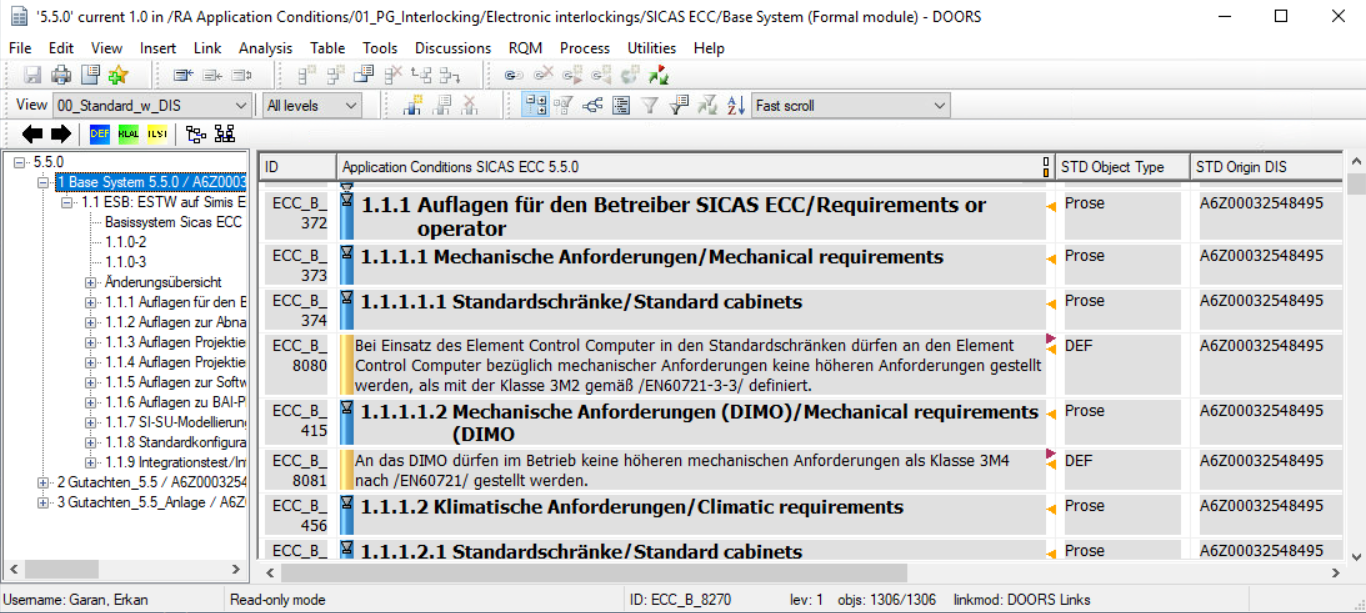
\includegraphics[width = \textwidth]{abbildungen/Modul in Doors.PNG}
    \caption{Geöffnetes Modul in \ac{DOORS}}
    \label{fig:Modul Doors}
\end{figure}


\subsection{Objekte und Attribute}
Innerhalb eines Moduls werden Daten in Objekten gespeichert. In der Regel bestehen Objekte aus mindestens zwei Spalten. Die erste 
Spalte enthält eine ID, die sich aus einem Präfix und einem Integerwert zusammensetzt. Der Integerwert wird bei jedem neu angelegtem 
Objekt inkrementiert, so dass jedem Objekt innerhalb eines Moduls eine eindeutige ID zugeordnet werden kann.
Die zweite Spalte besteht dabei entweder aus einer Sektions-Nummer und einer Überschrift, wie im ersten Objekt in der Abbildung 
\ref*{fig:Modul Doors} zu sehen ist, oder aus einem Objekt Text, der bspw. eine Anforderung beinhalten kann. Ein Beispiel für 
einen Objekt Text, der eine Anforderung beinhaltet ist das vierte Objekt der Abbildung \ref*{fig:Modul Doors} \cite[S.178]{DOORS}.
Einem Objekt können beliebig viele weitere Attribute hinzugefügt werden. 

Attribute beinhalten relevante Informationen über Module oder Objekte. Modulattribute speichern Informationen über das Modul, wie bspw.
den Ersteller des Moduls, das letzte Änderungsdatum und Ähnliches. Diese Modulattribute findet der User über die Eigenschaften des Moduls, 
welche mit einem Rechtsklick auf das Modul in der grafischen Oberfläche geöffnet werden können. Objektattribute hingegen
speichern Informationen über die Objekte. In der Abbildung \ref*{fig:Modul Doors} ist die Spalte STD Object Type z.B. ein Objektattribut,
das definiert, ob es sich bei dem Objekt um eine Anforderung oder um Prosa, also z.B. eine Überschrift handelt.

\subsection{Baseline}
Eine Baseline friert den aktuellen Stand der Anforderungen eines Projekts mit ihren Attributen ein und ist eine nicht veränderbare Kopie von 
formalen Modulen \cite[S.182]{DOORS}. Baselines werden in der Regel zu Releases von Systemen oder Subsystemen erstellt \cite[S.60]{RM-PE}. 
Wenn ein Formal Module geöffnet ist, kann der User unter File \textrightarrow{} Baseline eine Baseline erstellen oder eine bereits vorhandene 
Baseline ansehen. Abbildung \ref*{fig:Baselines} zeigt das Dialogfenster zum Öffnen bereits vorhandener Baselines. Dort wird deutlich, 
dass Baselines versioniert werden können.

\begin{figure}[h]
    \centering
    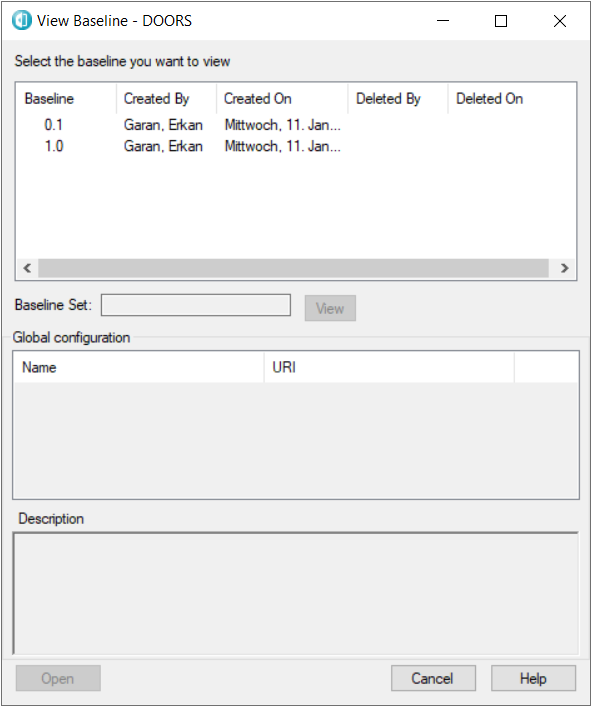
\includegraphics[width = \textwidth]{abbildungen/Baselines.PNG}
    \caption{Baselines eines Moduls in \ac{DOORS}}
    \label{fig:Baselines}
\end{figure}

\subsection{Links}
In der Abbildung \ref*{fig:Modul Doors} sind an der rechten Kante der zweiten Spalte zwei Arten von Pfeilen zu erkennen. Diese Pfeile
symbolisieren Links in \ac{DOORS}. Links sind gerichtete Verbindungen von einem Quellobjekt zu einem Zielobjekt. Sie werden in \ac{DOORS} 
genutzt, um die Verfolgbarkeit von Anforderungen zu gewährleisten. Der User kann 
dabei, ungeachtet von der Richtung des Links, vom Quellobjekt zum Zielobjekt oder auch andersherum navigieren \cite[S.183]{DOORS}. 
Ein nach links zeigender gelber Pfeil ist dabei ein In-Link, das heißt, dass dieses Objekt als Zielobjekt dient und ein anderes Objekt 
eine Verbindung zu diesem Objekt hat. Das Gegenstück zum In-Link ist ein Out-Link. Dieser wird in der grafischen Benutzeroberfläche von 
\ac{DOORS} als roter nach rechts zeigender Pfeil dargestellt. Hat ein Objekt einen Out-Link, heißt das, dass dieses Objekt als Quellobjekt 
dient und eine Verbindung zu einem anderem Objekt, welches als Zielobjekt dient, hat.   

\subsection{DXL}

\ac*{DXL} ist eine Skript-Sprache, die speziell für das Anforderungsmanagement-Tool \ac{DOORS} entwickelt wurde. Durch diese Skript-Sprache
besteht die Möglichkeit, die grafische Benutzeroberfläche von \ac{DOORS} um neue entwickelte Anwendungen zu
erweitern. Von der Syntax ähnelt die Sprache den Programmiersprachen C und C++ \cite[S.1]{DXL}. Zudem können Skripte geschrieben werden,
die als Batch-Script ausgeführt werden können. Diese Skripte bieten neben der grafischen Benutzeroberfläche eine weitere Möglichkeit, 
um mit \ac{DOORS} zu arbeiten. 
